\section{Comparative statics in cost without functional forms}\label{sec:03-revenue-tests}

Sumner's test in \cref{sec:03-sumner} turns a cost shock into a statement about conduct. It does so by
assuming a demand curve with constant elasticity and a flat marginal cost. This section studies three tests
that drop those functional forms. Each test asks what profit maximization alone implies about the response
of an equilibrium to a change in cost. The answers are inequalities. They can reject monopoly or bound
conduct from above, but they rarely deliver a point estimate.

We proceed in three steps. We first derive the bound of \citet{Sullivan1985} and explain why cost shifters
can only produce inequalities. We then prove the revealed-preference test of \citet{AshenfelterSullivan1987}
and report its evidence from the cigarette industry. Finally we develop the revenue test of
\citet{PanzarRosse1987}, which needs data on revenue and factor prices only.

\subsection{Sullivan's bound and why cost shifters give only inequalities}\label{sec:03-sullivan}

Consider $N$ firms selling a homogeneous good. Inverse demand $P(Q)$ is stable and decreasing, $P' < 0$.
Firm $i$ has cost $C_i(q_i) + t q_i$, where $t$ is a specific tax paid by sellers and $C_i$ is increasing.
Its marginal cost is therefore $MC_i = C_i'(q_i) + t \ge t$. Following \citet[eq.~24]{Bresnahan1989}, we
write the first-order condition of firm $i$ in conjectural-variations form,
\begin{equation}\label{eq:03-cv-foc}
  P(Q) + (1 + r_i)\, q_i P'(Q) = MC_i, \qquad i = 1, \dots, N,
\end{equation}
where $r_i$ is the conjectural variation $\frac{\dd Q_{-i}}{\dd q_i}$ of \cref{sec:03-objects}. Cournot behavior is
$r_i = 0$, joint profit maximization by $N$ identical firms is $1 + r_i = N$, and price taking is the limit
$1 + r_i \to 0$. As in \cref{sec:03-objects}, $r_i$ describes how close output is to the competitive and
collusive levels. It makes no claim about what firms believe.

\begin{definition}[Numbers equivalent]\label{def:03-numbers-equivalent}
Suppose $1 + r_i > 0$ for every $i$. The \emph{numbers equivalent} of the industry is
\begin{equation*}
  N_e = \sum_{i=1}^{N} \frac{1}{1 + r_i}.
\end{equation*}
\end{definition}

In a Cournot industry $N_e = N$, so $N_e$ counts the Cournot firms that would produce the same conduct. A
cartel of $N$ identical firms has $N_e = N \cdot \frac{1}{N} = 1$, and price taking corresponds to $N_e \to
\infty$. The next lemma connects $N_e$ to the industry conduct parameter of \eqref{eq:03-supply-relation}.

\begin{lemma}\label{lem:03-cv-aggregation}
If all firms have the same marginal cost $c$, the conditions \eqref{eq:03-cv-foc} aggregate to the supply
relation $P + \theta Q P'(Q) = c$ with $\theta = \frac{1}{N_e}$.
\end{lemma}

\begin{proof}
Rearrange \eqref{eq:03-cv-foc} as $P - c = -(1 + r_i) q_i P'$ and divide by $1 + r_i$:
\begin{equation*}
  \frac{P - c}{1 + r_i} = -q_i P'.
\end{equation*}
Summing over $i$ gives $(P - c) N_e = -Q P'$. Dividing by $N_e$ gives $P + \frac{1}{N_e} Q P' = c$.
\end{proof}

The lemma is a special case of \cref{prop:03-aggregation}. With a common marginal cost, each firm's condition reads
$s_i(1 + r_i) = \varepsilon\frac{P - c}{P}$, so every firm has the same value of $s_i\tilde\theta_i$. The industry
conduct $\sum_i \varphi_i s_i \tilde\theta_i$ is then the same for all weights, and the lemma shows that it equals
$\frac{1}{N_e}$.

Now let $z_c > 0$ be any variable that shifts marginal cost and is excluded from demand. The tax is the
leading example, and a factor price is another. Write the equilibrium price and output as $P^*(z_c)$ and
$Q^*(z_c)$. The \emph{reduced-form elasticities} of price and quantity with respect to the cost shifter are
\begin{equation}\label{eq:03-EP-EQ}
  E_P = \frac{\dd \ln P^*}{\dd \ln z_c}, \qquad E_Q = \frac{\dd \ln Q^*}{\dd \ln z_c}.
\end{equation}
\citet{Bresnahan1989} writes them $H_P$ and $H_Q$. Both can be estimated from regressions of log price and log
output on the cost shifter. The first result says what they reveal.

\begin{lemma}[Cost shifters trace out demand]\label{lem:03-trace-demand}
If $z_c$ does not enter demand and $E_P \neq 0$, the demand elasticity at the observed equilibrium is
$\varepsilon = -\frac{E_Q}{E_P}$, whatever the conduct, the slope of marginal cost and the curvature of
demand.
\end{lemma}

\begin{proof}
Every equilibrium lies on the same demand curve, so $P^*(z_c) = P(Q^*(z_c))$ for all $z_c$. Differentiating
in $z_c$ gives $\frac{\dd P^*}{\dd z_c} = P'(Q^*)\frac{\dd Q^*}{\dd z_c}$. Multiply both sides by
$\frac{z_c}{P^*}$ and insert $\frac{Q^*}{Q^*}$:
\begin{equation*}
  E_P = \frac{Q^* P'(Q^*)}{P^*} \cdot \frac{z_c}{Q^*}\frac{\dd Q^*}{\dd z_c} = -\frac{1}{\varepsilon}\, E_Q .
\end{equation*}
Solving for $\varepsilon$ completes the proof.
\end{proof}

\begin{proposition}[Sullivan's bound]\label{prop:03-sullivan-bound}
Suppose $1 + r_i > 0$ and $MC_i \ge t$ for every firm, and let $z_c$ satisfy \cref{lem:03-trace-demand}. Then
\begin{equation}\label{eq:03-sullivan-bound}
  N_e \;\ge\; \frac{1}{\varepsilon\left(1 - \frac{t}{P}\right)} \;=\; -\frac{E_P}{E_Q}\cdot\frac{P}{P - t}.
\end{equation}
If, in addition, all firms share the marginal cost $c$, conduct satisfies
\begin{equation}\label{eq:03-sullivan-theta}
  \theta = \varepsilon L = -L\,\frac{E_Q}{E_P} \;\le\; -\frac{E_Q}{E_P}\left(1 - \frac{t}{P}\right).
\end{equation}
\end{proposition}

\begin{proof}
By \eqref{eq:03-cv-foc}, $P - MC_i = -(1 + r_i) q_i P' > 0$, so $P > MC_i \ge t$. Divide by $1 + r_i > 0$ and
use $MC_i \ge t$:
\begin{equation*}
  \frac{P - t}{1 + r_i} \;\ge\; \frac{P - MC_i}{1 + r_i} \;=\; -q_i P'.
\end{equation*}
Sum over $i$ and use $-QP' = \frac{P}{\varepsilon}$:
\begin{equation*}
  (P - t)\, N_e \;\ge\; -Q P' \;=\; \frac{P}{\varepsilon}.
\end{equation*}
Divide by $P - t > 0$ to get $N_e \ge \frac{P}{\varepsilon (P - t)}$, which is the first expression in
\eqref{eq:03-sullivan-bound}. Substituting $\varepsilon = -\frac{E_Q}{E_P}$ from \cref{lem:03-trace-demand}
gives the second. Under a common marginal cost, \cref{lem:03-cv-aggregation} gives $\theta = \frac{1}{N_e}$
and \eqref{eq:03-lerner-theta} gives $\theta = \varepsilon L$. Finally $c \ge t$ implies $L \le 1 -
\frac{t}{P}$.
\end{proof}

Three features of the bound matter for what follows. First, it uses two reduced-form elasticities and the
tax share of the price. Nothing depends on the curvature of demand, the slope of marginal cost or the
functional form of either. Second, it is one-sided. A large value of the right side of
\eqref{eq:03-sullivan-bound} rejects collusive conduct, but no value can reject competition, because $N_e =
\infty$ satisfies every lower bound. Third, it is the Lerner bound \eqref{eq:03-lerner-bound} of
\cref{sec:03-sumner-replication} with the demand elasticity estimated from the cost shock itself.

\citet[eq.~25]{Bresnahan1989} states the bound in the form
\begin{equation*}
  \sum_i (1 + r_i)^{-1} \;\ge\; -\frac{H_P}{H_Q L} \;\ge\; -\frac{H_P}{H_Q},
\end{equation*}
with $H_P$ and $H_Q$ our $E_P$ and $E_Q$ and $L$ the common Lerner index. The first relation holds with
equality under a common marginal cost, by \cref{lem:03-cv-aggregation}. The second uses only $L \le 1$, that
is $MC \ge 0$, and coincides with \eqref{eq:03-sullivan-bound} at $t = 0$. Using the tax as a floor on
marginal cost tightens the bound, and this is the refinement that Sullivan uses
\citep[p.~1038]{Bresnahan1989}. For a cartel ($N_e = 1$) the bound says that $\varepsilon(1 - \frac{t}{P})
\ge 1$. A monopolist never prices on the inelastic part of demand, and the tax sharpens that rule. Its Lerner
index $\frac{1}{\varepsilon}$ cannot exceed the share of the price left after tax.

\begin{example}[An illustrative calculation]\label{ex:03-sullivan}
Suppose a 10 percent tax increase raises the price by 4 percent and lowers sales by 1.6 percent. Suppose
also that the tax is 40 percent of the price. These numbers are illustrative only. Then $E_P = 0.4$, $E_Q =
-0.16$ and $\varepsilon = \frac{0.16}{0.4} = 0.4$. The bound is
\begin{equation*}
  N_e \;\ge\; \frac{1}{0.4 \times (1 - 0.4)} = \frac{1}{0.24} \approx 4.2,
  \qquad \theta \;\le\; 0.24 .
\end{equation*}
Monopoly and Cournot conduct with up to four firms are rejected. Cournot conduct with five or more firms
is not.
\end{example}

\citet{Sullivan1985} applies the bound to a panel of U.S. states and years in the cigarette industry. State
excise taxes are the cost shifter, and an analysis-of-variance procedure absorbs the other exogenous
variables. He rejects the hypothesis that cigarette prices are set as if by a cartel
\citep[p.~1038]{Bresnahan1989}. \citet[p.~496]{AshenfelterSullivan1987} summarize his finding as industry
behavior inconsistent with a numbers equivalent below two or three.

\casehead{Why cost shifters give only inequalities} The proof of \cref{lem:03-trace-demand} shows what a
cost shifter does. Demand does not move, so every observed equilibrium lies on one demand curve, and
variation in $z_c$ traces that curve out. A cost shifter therefore identifies the demand elasticity at each
observed point. Conduct, however, sits in the supply relation, which in Lerner form reads $P - MC =
\theta\frac{P}{\varepsilon}$. Once $\varepsilon$ is known, $\theta$ is pinned down only if the level of
marginal cost is known. The data restrict it only to $t \le MC \le P$. Mapping these two bounds through the
supply relation gives the identified set
\begin{equation}\label{eq:03-cost-identified-set}
  0 \;\le\; \theta \;\le\; \varepsilon\left(1 - \frac{t}{P}\right).
\end{equation}
A demand shifter works the other way round. It moves equilibria along the supply relation and so traces out
the equation that contains $\theta$. \citet[p.~1039]{Bresnahan1989} draws this contrast, and
\cref{sec:03-identification} shows when demand shifters identify conduct. Pass-through is a partial
exception. The slope of price in cost does involve $\theta$, but \cref{prop:03-passthrough-id} shows that it
confounds conduct with the curvature of demand and the slope of marginal cost.

\subsection{Ashenfelter and Sullivan (1987): a revealed-preference test}\label{sec:03-ashenfelter-sullivan}

\casehead{Question} Parametric tests of monopoly fit equations of a chosen functional form and then test
restrictions on them. \citet{AshenfelterSullivan1987} point out that such a procedure always tests a joint
hypothesis. They quote \citet[p.~99]{Varian1983}: such a procedure tests ``whatever one wants to test plus
the maintained hypothesis of functional form.'' They therefore adapt the nonparametric
revealed-preference approach of \citet{Afriat1967} and \citet{Varian1982} to monopoly. Excise taxes are
well suited to it. Large tax changes give the test power, and every tax change yields a separate prediction.
The researcher can therefore report the percentage of correct predictions, which separates a model that
fails as a rule from one that fails occasionally (p.~484).

\casehead{The test} An industry acts as a single decision maker, a monopoly or a perfect cartel. It faces a
decreasing inverse demand $P(q)$ and a cost $C(q) = C_0(q) + tq$, where $C_0$ is increasing and $t$ is the
excise tax per unit. Let $t_0 < t_1$ be two tax rates with the same $P$ and $C_0$. Let $q_0$ and $q_1$ be the
profit-maximizing outputs and $p_0 = P(q_0)$, $p_1 = P(q_1)$ the prices.

\begin{proposition}[Ashenfelter and Sullivan]\label{prop:03-as-inequality}
Under these assumptions:
\begin{enumerate}[label=(\roman*)]
  \item Output does not rise and price does not fall, $q_1 \le q_0$ and $p_1 \ge p_0$.
  \item Revenue falls by at least the old tax times the fall in output,
  \begin{equation}\label{eq:03-as-revenue}
    p_1 q_1 - p_0 q_0 \;\le\; t_0\,(q_1 - q_0).
  \end{equation}
  \item If $p_1 > p_0$, the arc elasticity of demand satisfies
  \begin{equation}\label{eq:03-as-arc}
    \frac{(q_0 - q_1)\, p_0}{(p_1 - p_0)\, q_0} \;\ge\; \frac{p_0}{p_1 - t_0}.
  \end{equation}
\end{enumerate}
\end{proposition}

\begin{proof}
Output $q_0$ is optimal at tax $t_0$, so it earns at least as much as $q_1$ would:
\begin{equation}\label{eq:03-as-rp0}
  p_0 q_0 - C_0(q_0) - t_0 q_0 \;\ge\; p_1 q_1 - C_0(q_1) - t_0 q_1 .
\end{equation}
Output $q_1$ is optimal at tax $t_1$:
\begin{equation}\label{eq:03-as-rp1}
  p_1 q_1 - C_0(q_1) - t_1 q_1 \;\ge\; p_0 q_0 - C_0(q_0) - t_1 q_0 .
\end{equation}
Add the two inequalities. Revenues and the $C_0$ terms cancel, which leaves
\begin{equation*}
  -t_0 q_0 - t_1 q_1 \;\ge\; -t_0 q_1 - t_1 q_0
  \quad\Longleftrightarrow\quad
  (t_1 - t_0)(q_0 - q_1) \;\ge\; 0 .
\end{equation*}
Since $t_1 > t_0$, $q_1 \le q_0$. Demand slopes down, so $p_1 \ge p_0$. This proves (i). Rearrange
\eqref{eq:03-as-rp0}:
\begin{equation*}
  p_1 q_1 - p_0 q_0 \;\le\; \bigl[C_0(q_1) - C_0(q_0)\bigr] + t_0 (q_1 - q_0).
\end{equation*}
The bracket is not positive because $q_1 \le q_0$ and $C_0$ is increasing. This proves (ii). For (iii),
write $p_1 q_1 - p_0 q_0 = p_1(q_1 - q_0) + q_0(p_1 - p_0)$ and substitute into \eqref{eq:03-as-revenue}:
\begin{equation*}
  q_0 (p_1 - p_0) \;\le\; (p_1 - t_0)(q_0 - q_1).
\end{equation*}
A monopolist prices above marginal cost, so $p_1 > t_1 > t_0$. Multiply both sides by the positive number
$\frac{p_0}{q_0 (p_1 - p_0)(p_1 - t_0)}$ to obtain \eqref{eq:03-as-arc}.
\end{proof}

Inequality \eqref{eq:03-as-revenue} has a direct reading. Moving from $q_0$ to $q_1$ saves $t_0(q_0 - q_1)$
in taxes at the old rate. The revenue lost by the move must exceed this saving. Otherwise the monopolist
would have chosen $q_1$ when the tax was still $t_0$. Inequality \eqref{eq:03-as-arc} extends the rule that a
monopolist never produces on the inelastic part of demand. The arc elasticity must exceed
$\frac{p_0}{p_1 - t_0}$, which is above one whenever the price rises by less than the old tax. The test uses
two observed points, no functional form, no derivatives and no convexity of cost. It is local because it
compares points close in time, where demand and cost are plausibly the same. \Cref{fig:03-as-test} draws the
logic in the plane of output and revenue.

\begin{figure}[htbp]
\centering
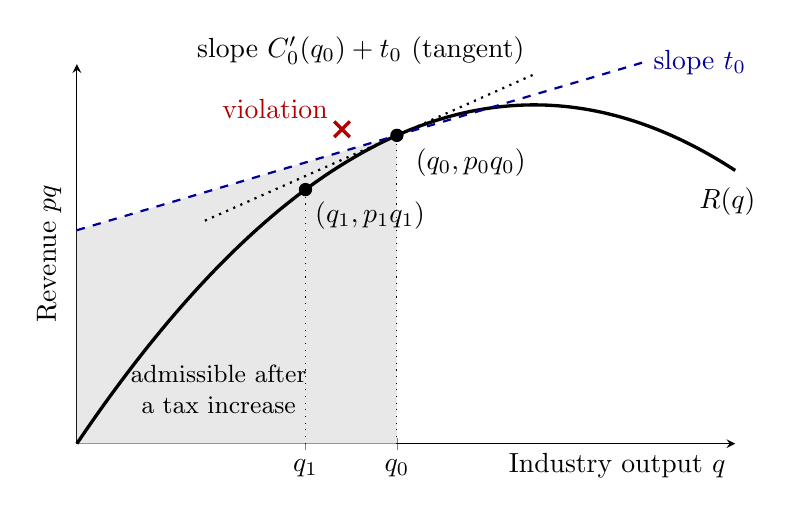
\begin{tikzpicture}
\begin{axis}[
  width=0.82\textwidth, height=6.4cm,
  xmin=0, xmax=7.2, ymin=0, ymax=28,
  axis lines=left,
  xlabel={Industry output $q$}, ylabel={Revenue $pq$},
  xtick={2.5,3.5}, xticklabels={$q_1$,$q_0$},
  ytick=\empty, clip=false,
  every axis x label/.style={at={(ticklabel* cs:1.0)}, anchor=north east}
]
  \addplot[fill=gray!18, draw=none] coordinates {(0,0) (0,15.75) (3.5,22.75) (3.5,0)} -- cycle;
  \addplot[domain=0:7.2, samples=120, very thick, black] {10*x - x^2};
  \node[anchor=north west] at (axis cs:6.7,19.6) {$R(q)$};
  \addplot[domain=0:6.2, thick, dashed, blue!60!black] {22.75 + 2*(x - 3.5)};
  \node[anchor=west, blue!60!black] at (axis cs:6.2,28.15) {slope $t_0$};
  \addplot[domain=1.4:5.0, thick, dotted, black] {22.75 + 3*(x - 3.5)};
  \node[anchor=south east] at (axis cs:5.0,27.25) {slope $C_0'(q_0) + t_0$ (tangent)};
  \addplot[only marks, mark=*, mark size=2.2pt] coordinates {(3.5,22.75) (2.5,18.75)};
  \node[anchor=north west] at (axis cs:3.6,22.5) {$(q_0, p_0 q_0)$};
  \node[anchor=north west] at (axis cs:2.5,18.6) {$(q_1, p_1 q_1)$};
  \addplot[only marks, mark=x, mark size=4pt, very thick, red!70!black] coordinates {(2.9,23.2)};
  \node[anchor=south east, red!70!black] at (axis cs:2.85,23.3) {violation};
  \draw[dotted] (axis cs:3.5,0) -- (axis cs:3.5,22.75);
  \draw[dotted] (axis cs:2.5,0) -- (axis cs:2.5,18.75);
  \node[anchor=center, align=center, font=\small] at (axis cs:1.55,4.0) {admissible after\\ a tax increase};
\end{axis}
\end{tikzpicture}
\caption{The revealed-preference logic of \cref{prop:03-as-inequality}. After the tax rises from $t_0$ to
$t_1$, the new point $(q_1, p_1q_1)$ must lie left of $q_0$ and below the line through $(q_0, p_0q_0)$ with
slope $t_0$ (shaded region). The tangent of the revenue curve at $q_0$ has slope equal to marginal revenue,
$C_0'(q_0) + t_0$, which is at least $t_0$. A point above the dashed line, such as the cross, rejects monopoly
with stable demand and cost. The curve is drawn for $R(q) = 10q - q^2$, $C_0' = 1$, $t_0 = 2$ and $t_1 =
4$.}
\label{fig:03-as-test}
\end{figure}

\casehead{A conduct index} The test extends to intermediate conduct. Following
\citet[eq.~12]{AshenfelterSullivan1987}, who call the index $\beta$, say that the industry has
\emph{conduct index} $\theta \in [0, 1]$ if, at its chosen output $q$,
\begin{equation}\label{eq:03-as-index}
  \Delta q\, P(q + \Delta q) + \theta\, q \bigl[P(q + \Delta q) - P(q)\bigr] \;\le\; C(q + \Delta q) - C(q)
  \quad \text{for all } \Delta q .
\end{equation}
With $\theta = 1$ the left side equals $(q + \Delta q)P(q + \Delta q) - qP(q)$, so \eqref{eq:03-as-index} is the
monopoly optimality condition. With $\theta = 0$ it is the revealed-preference form of price equal to marginal
cost. Dividing \eqref{eq:03-as-index} by $\Delta q > 0$ and letting $\Delta q \to 0$ gives $P + \theta q P'
\le C'$. Dividing by $\Delta q < 0$ reverses the inequality. Together they give $P + \theta q P' = C'$, which is
the supply relation \eqref{eq:03-supply-relation}. The index is therefore a finite-difference version of the
conduct parameter.

Apply \eqref{eq:03-as-index} at $q = q_0$ under tax $t_0$ with $\Delta q = q_1 - q_0$. Then drop the term
$C_0(q_1) - C_0(q_0) \le 0$. For $\theta \in (0, 1)$ the signs $q_1 \le q_0$ and $p_1 \ge p_0$ can no longer
be proved, so the test assumes them (p.~487). Under these signs,
\begin{equation*}
  p_1 (q_1 - q_0) + \theta\, q_0 (p_1 - p_0) \;\le\; t_0 (q_1 - q_0).
\end{equation*}
Solving for $\theta$ and inverting gives the two forms of the bound
\begin{equation}\label{eq:03-as-ne}
  \theta \;\le\; \frac{(p_1 - t_0)(q_0 - q_1)}{(p_1 - p_0)\, q_0},
  \qquad
  N_e = \frac{1}{\theta} \;\ge\; \frac{q_0 (p_1 - p_0)}{(q_0 - q_1)(p_1 - t_0)} .
\end{equation}
The second form is the arc version of \eqref{eq:03-sullivan-bound}.\footnote{\citet[eq.~18]{AshenfelterSullivan1987}
derive the bound on $N_e$ separately, by integrating the firms' first-order conditions over the tax change.
Their printed equation has $q_1 - q_0$ in the denominator. We reverse that factor so that the bound is
positive, as their equation (14) and their text require.} To see this, evaluate the elasticities at
some price $p$ between $p_0$ and $p_1$. Then $-\frac{E_P}{E_Q}$ becomes the ratio of the percentage price
rise to the percentage output fall, $\frac{q_0 (p_1 - p_0)}{p\,(q_0 - q_1)}$. The factor $\frac{P}{P - t}$
becomes $\frac{p}{p_1 - t_0}$, because $p_1 - t_0$ bounds the per-unit margin from above along the path.
Multiplying the two gives the right side of \eqref{eq:03-as-ne}. Like Sullivan's bound, \eqref{eq:03-as-ne} can only reject less
competitive conduct in favor of more competitive conduct (their n.~6).

\casehead{Data} The data are those of \citet{Sullivan1985}, from the Tobacco Tax Council's \emph{The Tax
Burden on Tobacco}. They cover 45 states from 1955 to 1982 and contain three variables. The tax is the sum of
the state and federal excise rates, averaged by time in force in years when the rate changed. Per capita
consumption is inferred from state tax receipts. The average retail price per pack comes from a survey taken
each November. Both dollar variables are deflated by the national consumer price index. The industry is
highly concentrated. It has six major firms, and the two and four largest firms produce 66 and 90 percent of
output. The major firms kept virtually identical list prices for thirty years and were twice convicted of
antitrust violations (p.~488).

\casehead{Design} Demand and cost may differ across states and drift over time. The test is therefore applied
only to pairs of observations from the same state at most two years apart. Each pair is ordered so that
$t_0$ is the lower real tax rate. The authors consider all consecutive-year pairs and several subsets. They
also use \emph{skip-year} pairs, separated by one year, which avoid the time-averaged tax in years of
change. The cleanest subset is \emph{flat-jump-flat}: the statutory rate is constant in both years of the
pair and rises in the year between them. For each pair they check the output and price predictions of
\cref{prop:03-as-inequality}(i) and the revenue inequality \eqref{eq:03-as-revenue}.

\begin{table}[htbp]
\centering
\caption{Ashenfelter and Sullivan (1987): percentage of monopoly predictions that hold}
\label{tab:03-as-tests}
\begin{tabular}{lrccccc}
\toprule
 & & \multicolumn{5}{c}{Percentage of pairs for which the prediction holds} \\
\cmidrule(lr){3-7}
Pairs of observations & Cases & $\Delta q \le 0$ & $\Delta p \ge 0$ & Both & Revenue & All three \\
\midrule
\multicolumn{7}{l}{\textit{Panel A: Table I}} \\
Consecutive years & 1178 & 70.8 & 75.3 & 54.6 & 36.7 & 14.9 \\
\quad real tax increases & 216 & 74.1 & 83.8 & 68.1 & 17.1 & 6.0 \\
\quad real tax decreases & 962 & 70.1 & 73.4 & 51.6 & 41.1 & 16.8 \\
\quad statutory changes & 288 & 69.8 & 81.9 & 62.5 & 22.9 & 9.7 \\
\quad no statutory change & 890 & 71.1 & 73.2 & 52.0 & 41.1 & 16.5 \\
Skip-year changes & 1133 & 71.8 & 85.0 & 62.0 & 27.4 & 15.1 \\
\quad flat-jump-flat & 199 & 68.8 & 94.0 & 66.8 & 13.6 & 10.6 \\
\addlinespace
\multicolumn{7}{l}{\textit{Panel B: Table II, skip-year changes by size of the tax change}} \\
$\Delta t < 1$ cent & 467 & 69.2 & 76.9 & 53.5 & 42.0 & 23.1 \\
$1 < \Delta t < 2$ cents & 444 & 69.1 & 86.9 & 61.0 & 23.0 & 11.9 \\
$\Delta t > 2$ cents & 222 & 82.9 & 98.2 & 81.5 & 5.9 & 4.5 \\
\bottomrule
\end{tabular}

\smallskip
\begin{minipage}{0.95\textwidth}
\footnotesize Notes: Reproduced from \citet[Tables I and II]{AshenfelterSullivan1987}. ``Revenue'' is
inequality \eqref{eq:03-as-revenue}. ``Both'' requires output to fall and price to rise. ``All three'' adds
the revenue inequality. In each pair the lower real tax rate defines $t_0$. Tax changes in Panel B are in 1967
cents. The paper's Table II labels the last row $\Delta t < 2$, but its text (pp.~491--492) identifies the row
as changes above 2 cents, and the three rows sum to the 1133 skip-year cases. Its first column header reads
$\Delta q \ge 0$, while its note defines the prediction as a decline in quantity.
\end{minipage}
\end{table}

\casehead{Results} \Cref{tab:03-as-tests} reproduces the main results. The revenue inequality, the
distinctive prediction of monopoly, holds in only 432 of 1178 consecutive-year pairs, or 36.7 percent. It
fares worse where measurement is cleanest. It holds in 13.6 percent of the flat-jump-flat pairs and in only
5.9 percent of the skip-year pairs with tax changes above 2 cents.
The output and price predictions also fail often. They hold jointly in 54.6 percent of all consecutive-year
pairs. They improve with the size of the tax change, to 81.5 percent for changes above 2 cents. The pattern
is the one the authors stress (p.~492). Large tax increases usually raise prices and lower sales, yet they
rarely lower revenue by as much as monopoly requires.

\Cref{fig:03-as-numbers} asks which oligopoly conduct the data can rationalize. It applies the bound
\eqref{eq:03-as-ne} to the pairs in which output fell and price rose. These are 702 skip-year pairs and 133
flat-jump-flat pairs. Only 24.4 and 15.8 percent of them are consistent with $N_e = 1$. A numbers equivalent of
5 rationalizes 75.1 and 76.7 percent. Even $N_e = 9$ leaves 13.5 and 12.0 percent unexplained. The authors
conclude that simple conjectural-variations models can be rejected ``unless they embody at least a moderate
amount of competition'' (p.~492).

\begin{figure}[htbp]
\centering
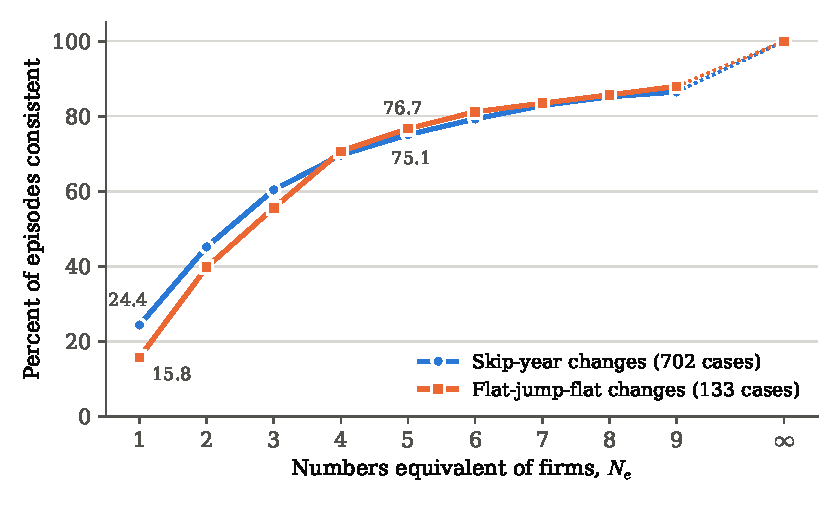
\includegraphics[width=0.78\textwidth]{figures/ch03/as_numbers_equivalent.pdf}
\caption{Share of tax-increase episodes consistent with a numbers equivalent $N_e$, from the bound
\eqref{eq:03-as-ne}. Only pairs with $\Delta q \le 0$ and $\Delta p \ge 0$ enter. At $N_e = \infty$ every
episode is consistent. The paper's table heads the second column ``Jump-Flat-Jump'', and its text calls the
sample flat-jump-flat. Redrawn from the numbers in \citet[Table III]{AshenfelterSullivan1987}.}
\label{fig:03-as-numbers}
\end{figure}

\casehead{Robustness} The authors probe the failures in four ways. First, 371 of the 1133 skip-year pairs
show price and quantity moving in the same direction, which signals a demand shift. Dropping them raises both
the output and the price predictions to 92 percent, while the revenue inequality holds in only 26 percent
(p.~493). Second, they allow for trends with a comparison group. In a simple version, the predicted change without a
tax change is the mean change in states that kept their statutory rate that year. In a two-way version, it is
the fit of a model with state and year effects to the state-years without a statutory change. The tests then ask whether quantity fell below, and price
rose above, these predictions. Their Table IV reports the results. With the simple fit, the quantity and price
predictions hold in 68.4 and 80.9 percent of the 288 consecutive-year statutory changes, and jointly in 60.1
percent. On the 199 flat-jump-flat pairs they hold in 68.8 and 92.0 percent, and jointly in 65.3 percent. The
two-way fit does better. On the statutory changes the shares are 77.8, 79.2 and 68.4 percent. On flat-jump-flat
pairs both predictions hold in 83.9 percent of cases, with 85.9 and 97.0 percent separately. The authors note the analogy with
program evaluation, where untreated units serve as controls \citep{Ashenfelter1978}. In modern terms this is a
difference-in-differences adjustment (\cref{app:econometrics}). Third, in nominal terms the price rises in 196
of the 199 flat-jump-flat pairs, though rising consumer prices make that success partly mechanical. Fourth,
they test whether tax increases follow particular movements in prices and quantities. Their sign-based
contingency tables condition on whether the tax rose in the previous year. The Pearson statistic is 3.9 when it
did not and 34.9 when it did, each with 3 degrees of freedom. The overall statistic is 38.8 with 6 degrees of
freedom. The second and the overall statistic rest on cells with very small expected counts, so the
$\chi^2$ approximation may be poor. Almost all of the 34.9 comes from the two cells in which price and quantity
both fell. The authors conclude that endogenous tax timing does not explain the failures (Table V,
pp.~495--496).

\casehead{Assessment} The test shows how far pure revealed preference can go, and it rejects monopoly
decisively. Its limits are instructive. The approach has no stochastic framework, a drawback the authors
acknowledge (n.~3). The percentages are therefore descriptive, and a single mismeasured pair can violate
\eqref{eq:03-as-revenue}. Quantities
inferred from tax receipts are suspect in exactly the years the test uses, because consumers and retailers
can stock up before a tax increase or buy across state lines. The maintained hypothesis of stable demand and
cost over one or two years is strong, as the frequent failures of the output and price predictions show.
Once a comparison group corrects for demand shifts, the test is no longer nonparametric, as the authors
concede (p.~494). Finally, a rejection of monopoly says little about which oligopoly model holds, beyond the
lower bound on $N_e$. The paper's lasting contribution is the idea of bounding conduct with inequalities
implied by optimization, which returns in \cref{sec:03-bounds}.

\subsection{Panzar and Rosse (1987): the revenue test}\label{sec:03-panzar-rosse}

\citet{PanzarRosse1987} propose two ideas \citep[pp.~1034--1035]{Bresnahan1989}. The first is to estimate a
reduced form and focus on the coefficients of factor prices. The second is to use revenue as the dependent
variable. Revenue is often observable when price and quantity are not. It also needs no quality correction,
whereas a price per unit can overstate the true price where the product is better. \Cref{sec:01-id-cost} previewed
the test. This section proves its properties.

\casehead{Setup} Firm $i$ produces output $q$ at cost $C(q, w, z)$, where $w = (w_1, \dots, w_K)$ is the
vector of factor prices and $z$ collects other cost shifters. Its revenue function is $R(q, y)$, with $y$ a
vector of demand shifters. Solving the equilibrium for the firm's revenue gives the \emph{reduced-form
revenue} $R^*(w, z, y)$. The \emph{Panzar-Rosse statistic} is the sum of the factor-price elasticities of
reduced-form revenue,
\begin{equation}\label{eq:03-pr-psi}
  \psi = \sum_{k=1}^{K} \frac{\partial R^*}{\partial w_k}\frac{w_k}{R^*}
       = \frac{\dd \ln R^*(\lambda w, z, y)}{\dd \lambda}\bigg|_{\lambda = 1},
\end{equation}
where the second equality follows from the chain rule. In words, $\psi$ is the percentage change in
equilibrium revenue after a 1 percent increase in all factor prices. \citet{Bresnahan1989} writes it $H_R$.
With a log-linear specification,
\begin{equation}\label{eq:03-pr-regression}
  \ln R_i = a + \sum_{k=1}^{K} \beta_k \ln w_{ki} + \gamma^\top x_i + e_i, \qquad \hat\psi = \sum_{k=1}^{K}
  \hat\beta_k ,
\end{equation}
where $x_i$ contains the other cost and demand shifters. Early applications either use such a
specification, which makes $\psi$ constant, or report $\psi$ near the center of the sample
\citep[n.~27]{Bresnahan1989}.

\begin{lemma}[Homogeneity of cost]\label{lem:03-homogeneity}
For a cost-minimizing firm and every $\lambda > 0$, $C(q, \lambda w, z) = \lambda C(q, w, z)$. Marginal cost
$C_q$ is also homogeneous of degree one in $w$, and $\sum_k w_k \frac{\partial C_q}{\partial w_k} = C_q$.
\end{lemma}

\begin{proof}
Scaling all factor prices by $\lambda$ leaves relative prices, and hence the cost-minimizing input bundle,
unchanged. Cost is therefore multiplied by $\lambda$. Differentiating $C(q, \lambda w, z) = \lambda C(q, w,
z)$ in $q$ gives $C_q(q, \lambda w, z) = \lambda C_q(q, w, z)$. Euler's theorem for functions homogeneous of
degree one gives the last statement.
\end{proof}

\begin{proposition}[Panzar and Rosse]\label{prop:03-panzar-rosse}
\leavevmode
\begin{enumerate}[label=(\roman*)]
  \item \emph{Monopoly.} If the firm is a monopolist, $\psi \le 0$. This holds also when it chooses a vector
  of outputs, qualities or advertising levels.
  \item \emph{Long-run competition.} Suppose free entry drives every active firm to the minimum of a U-shaped
  average cost curve. Then $\psi = 1$, and firm revenue does not depend on the demand shifters $y$.
  \item \emph{Chamberlinian competition.} Consider a symmetric free-entry equilibrium in which each firm
  maximizes profit against a downward-sloping demand. Suppose entry shifts that demand down and does not make
  it less elastic at a given output. Then $\psi \le 1$.
\end{enumerate}
\end{proposition}

\begin{proof}
\emph{(i), first proof: revealed preference.} Let $x$ be the vector of choices, with revenue $R(x)$ and cost
$C(x, w)$ homogeneous of degree one in $w$. Fix $w^0$ and $w^1 = \lambda w^0$ with $\lambda > 1$, and let $x^0$
and $x^1$ be the optimal choices. Optimality of $x^0$ at $w^0$ gives
\begin{equation*}
  R(x^0) - C(x^0, w^0) \ge R(x^1) - C(x^1, w^0)
  \quad\Longrightarrow\quad
  C(x^1, w^0) - C(x^0, w^0) \ge R(x^1) - R(x^0).
\end{equation*}
Optimality of $x^1$ at $w^1$, with $C(x, w^1) = \lambda C(x, w^0)$, gives
\begin{equation*}
  R(x^1) - R(x^0) \;\ge\; \lambda\bigl[C(x^1, w^0) - C(x^0, w^0)\bigr] \;\ge\; \lambda\bigl[R(x^1) -
  R(x^0)\bigr],
\end{equation*}
where the second step uses the first display. Hence $(1 - \lambda)[R(x^1) - R(x^0)] \ge 0$. Since $\lambda >
1$, $R(x^1) \le R(x^0)$. Equilibrium revenue cannot rise when all factor prices rise in proportion, so
$R^*(\lambda w^0) \le R^*(w^0)$ for $\lambda > 1$, and \eqref{eq:03-pr-psi} gives $\psi \le 0$.

\emph{(i), second proof: comparative statics.} With a single output, the monopolist's first-order condition
is $R_q(q^*, y) = C_q(q^*, w, z)$, and the second-order condition is $R_{qq} - C_{qq} < 0$. Differentiating the
first-order condition in $w_k$ gives
\begin{equation*}
  R_{qq}\frac{\partial q^*}{\partial w_k} = C_{qq}\frac{\partial q^*}{\partial w_k} + C_{q w_k}
  \quad\Longrightarrow\quad
  \frac{\partial q^*}{\partial w_k} = \frac{C_{q w_k}}{R_{qq} - C_{qq}} .
\end{equation*}
Equilibrium revenue is $R^* = R(q^*(w), y)$, so $\frac{\partial R^*}{\partial w_k} = R_q \frac{\partial
q^*}{\partial w_k}$. Multiply by $w_k$, sum over $k$, and apply \cref{lem:03-homogeneity} and then the
first-order condition:
\begin{equation*}
  \sum_k w_k \frac{\partial R^*}{\partial w_k}
  = \frac{R_q \sum_k w_k C_{q w_k}}{R_{qq} - C_{qq}}
  = \frac{R_q\, C_q}{R_{qq} - C_{qq}}
  = \frac{(R_q)^2}{R_{qq} - C_{qq}} .
\end{equation*}
Dividing by $R^*$ yields
\begin{equation}\label{eq:03-pr-monopoly}
  \psi = \frac{(R_q)^2}{(R_{qq} - C_{qq})\, R^*} \;\le\; 0,
\end{equation}
which is equation (23) of \citet{Bresnahan1989}. The inequality is strict when marginal cost is positive,
because then $R_q > 0$.

\emph{(ii)} Write average cost as $AC(q, w, z) = \frac{C(q, w, z)}{q}$. Each active firm produces at the output
$q^m(w, z)$ that minimizes it, and free entry sets the price equal to minimum average cost $MAC(w, z)$. By
\cref{lem:03-homogeneity}, $AC(q, \lambda w, z) = \lambda AC(q, w, z)$. Scaling by $\lambda$ does not move the
minimizer, so $q^m$ is homogeneous of degree zero in $w$, and $MAC$ is homogeneous of degree one. Firm revenue
$R^* = MAC(w, z)\, q^m(w, z)$ is then homogeneous of degree one in $w$, and Euler's theorem gives $\sum_k w_k
\frac{\partial R^*}{\partial w_k} = R^*$, that is, $\psi = 1$. Neither factor of $R^*$ involves $y$. A demand
shift changes the number of firms and leaves the revenue of each unchanged.

\emph{(iii)} Treat the number of firms $n$ as continuous. Each firm's revenue is $R(q, n)$ with $R_n < 0$,
since more rivals lower the price at which a given output sells. A symmetric equilibrium satisfies
$R_q(q, n) = C_q(q, w)$ and zero profit, $R(q, n) = C(q, w)$. Scale $w$ by $\lambda$ and differentiate both
conditions at $\lambda = 1$, using $C(q, \lambda w) = \lambda C(q, w)$:
\begin{align*}
  R_q\, \dd q + R_n\, \dd n &= C_q\, \dd q + C\, \dd\lambda, \\
  R_{qq}\, \dd q + R_{qn}\, \dd n &= C_{qq}\, \dd q + C_q\, \dd\lambda .
\end{align*}
Since $R_q = C_q$, the first line gives $R_n\, \dd n = C\, \dd\lambda$. The change in revenue is $\dd R^* = R_q\, \dd q +
R_n\, \dd n = C_q\, \dd q + C\, \dd\lambda$. Dividing by $R^* = C$ gives
\begin{equation*}
  \psi = 1 + \frac{C_q}{C}\,\frac{\dd q}{\dd\lambda},
\end{equation*}
so $\psi \le 1$ exactly when firm output does not rise. Substituting $\frac{\dd n}{\dd\lambda} = \frac{C}{R_n}$
into the second line gives
\begin{equation*}
  \frac{\dd q}{\dd\lambda} = \frac{C_q - \frac{R_{qn}}{R_n}\, C}{R_{qq} - C_{qq}} .
\end{equation*}
The denominator is negative by the second-order condition. So $\frac{\dd q}{\dd\lambda} \le 0$ if and only if $C_q
\ge \frac{R_{qn}}{R_n}C$. Use $C = R$ and $C_q = R_q$, divide by $R > 0$, and multiply by
$\frac{R_n}{R_q} < 0$. The condition becomes $\frac{R_n}{R} \le \frac{R_{qn}}{R_q}$, that is,
$\frac{\partial}{\partial n}\ln\frac{R_q}{R} \ge 0$. At a fixed $q$, $\frac{q R_q}{R} = 1 -
\frac{1}{\varepsilon_f}$, where $\varepsilon_f$ is the elasticity of the firm's demand. The condition
therefore says that entry does not lower $\varepsilon_f$.
\end{proof}

Part (iii) is Proposition~1 of \citet[p.~451]{PanzarRosse1987}. They assume that each firm's inverse demand
falls with its own output and with the number of rivals. Their Assumption~1 adds that the elasticity of each
firm's perceived demand is nondecreasing in the number of symmetric rivals (p.~450). The derivation above is
ours. Like theirs, it shows that the result rests on how entry changes the elasticity of each firm's demand.
When entry leaves $\varepsilon_f$ unchanged, firm output is fixed and $\psi = 1$, as in the long-run
competitive case. Panzar and Rosse also show that monopolistic competition, long-run competition and
conjectural-variation oligopoly are each consistent with $\psi > 0$ (p.~447). In their oligopoly model, $\psi$
has the sign opposite to that of industry marginal revenue. It is positive when industry output lies on the
inelastic part of market demand (pp.~454--455).

\begin{example}[Values of $\psi$ in standard models]\label{ex:03-pr-examples}
Let marginal cost be a constant $c(w)$, homogeneous of degree one in $w$, so that $\frac{\dd\ln c}{\dd\ln\lambda}
= 1$.
\begin{enumerate}[label=(\alph*)]
  \item Monopoly with demand $Q = AP^{-\varepsilon}$, $\varepsilon > 1$. The price is $P =
  \frac{\varepsilon}{\varepsilon - 1}c$ and revenue is $R^* = AP^{1 - \varepsilon}$, so $\psi = 1 -
  \varepsilon < 0$.
  \item Monopoly with demand $P = a - bQ$. Then $Q = \frac{a - c}{2b}$, $P = \frac{a + c}{2}$ and $R^* =
  \frac{a^2 - c^2}{4b}$, so $\psi = -\frac{2c^2}{a^2 - c^2} < 0$.
  \item Long-run competition with $C(q, w) = g(w)(f + q^2)$ and $g$ homogeneous of degree one. Average cost
  $g(w)(\frac{f}{q} + q)$ is minimized at $q^m = \sqrt{f}$, so $MAC = 2g(w)\sqrt{f}$, $R^* = 2g(w)f$ and
  $\psi = 1$.
  \item Short-run competition with $n$ fixed firms and rising marginal cost. Firm revenue is $\frac{P\,
  D(P)}{n}$, so $\psi = (1 - \varepsilon)\frac{\dd\ln P}{\dd\ln\lambda}$. Its sign is the sign of $1 -
  \varepsilon$.
  \item Cournot with $n$ fixed firms and demand $Q = AP^{-\varepsilon}$, $n\varepsilon > 1$. The Lerner
  index is $\frac{1}{n\varepsilon}$, so $P = \frac{n\varepsilon}{n\varepsilon - 1}c$. Firm revenue is
  $\frac{AP^{1 - \varepsilon}}{n}$, so $\psi = 1 - \varepsilon$, as under monopoly.
\end{enumerate}
\end{example}

Cases (d) and (e) show what the statistic cannot do. Short-run competition and oligopoly do not sign $\psi$,
and $\psi < 0$ arises without monopoly whenever demand is elastic. A negative $\hat\psi$ is therefore no proof
of monopoly, a ``false finding of monopoly'' in the words of \citet[p.~1036]{Bresnahan1989}. The usable
conclusions are one-sided. An estimate $\hat\psi > 0$ rejects monopoly. An estimate $\hat\psi < 1$ rejects
long-run competition, provided the markets are in long-run equilibrium. An estimate between zero and one
rejects both.

The specification matters as much as the sign. When the hypothesis is monopoly, $R^*$ depends on demand
shifters, and the revenue equation is misspecified if they are left out \citep[n.~28]{Bresnahan1989}. When
the hypothesis is long-run competition, demand shifters should have zero coefficients. This gives a second
testable restriction (p.~1037 and n.~30). Every factor price must be measured, and each must vary
exogenously. If a factor is omitted, $\hat\psi$ measures the response to only part of a proportional cost
increase. The long-run interpretation also requires that a cross-section of local markets reflects
differences in long-run equilibria. \citet{Rosse1970} addresses this with a ``permanent plant'' hypothesis,
and markets with rising demand should be treated separately from markets with falling demand
\citep[p.~1037]{Bresnahan1989}.

\casehead{Applications} The first applications use cross-sections of similar local markets, which suits the
long-run reading of the statistic. In a newspaper study, \citet{PanzarRosse1977} take each newspaper as an
observation, with its revenue, mostly from advertising, as the dependent variable. They reject monopoly
($\hat\psi > 0$) even for newspapers that are the only paper in their town. \citet[p.~1037]{Bresnahan1989} reads
this as evidence of competition from other media. In all but one specification the study also rejects $\psi = 1$,
and no specification rejects the Chamberlinian bound $\psi \le 1$. \citet[p.~453, n.~4]{PanzarRosse1987} call these
results suggestive rather than conclusive. \citet{Shaffer1982} applies the test to a cross-section of
banks in New York State in 1979. He rejects both monopoly and long-run competition (p.~1037). The test also bears on market definition. A rejection of monopoly for a firm or a
group of firms means they cannot be treated as acting in isolation \citep[p.~1050]{Bresnahan1989}.

\casehead{Assessment} The revenue test asks little of the data on endogenous variables and makes no
assumption about functional forms. Its demands lie elsewhere. It needs the full vector of factor prices with
exogenous variation in each, and its sharpest prediction ($\psi = 1$) requires long-run equilibrium with free
entry. Like the two tests before it, it delivers inequalities. All three reject monopoly or cartel pricing in
their applications, and none of them says how much market power remains.

\section{Residual demand: Baker and Bresnahan (1988)}\label{sec:03-residual-demand}

\subsection{The question and the idea}\label{sec:03-rd-idea}

The tests so far treat the product as homogeneous and ask about industry conduct. Most industries sell
differentiated products, and then a firm's market power depends on substitution as well as on behavior. A
firm with a unique product can have substantial power, while a firm whose rival sells a near-identical
product may have almost none. Measuring this with a full demand system is costly. Even with constant
elasticities and symmetry, $N$ products require $N$ own-price elasticities, $N$ income elasticities and
$\frac{N(N - 1)}{2}$ cross-price elasticities \citep[p.~1045]{Bresnahan1989}. With 100 products that is more
than 5,000 parameters.

\citet{BakerBresnahan1988} estimate one equation per firm instead. The \emph{residual demand curve} of a firm
is the relation between its own price and quantity after accounting for the supply response of all other
firms (p.~284). A firm in a perfectly competitive industry faces a flat residual demand curve. A monopolist's
residual demand is the industry demand. A firm selling a differentiated product lies in between.
\Cref{fig:03-residual-demand} draws the construction for a homogeneous good. The slope of residual demand
summarizes market power without identifying its source.

\subsection{Deriving the residual demand curve}\label{sec:03-rd-model}

Firm 1 is the firm of interest and sells a single product. Let $\mathbf{Q} = (Q_2, \dots, Q_N)$ be the
quantities of all other relevant products, including products of firms in other ``industries''. No market
is defined in advance. Let $Y$ be demand shifters, $W$ industry-wide cost shifters, and $W^i$ cost shifters
specific to firm $i$. The model has four blocks \citep[pp.~286--289]{BakerBresnahan1988}. Firm 1's inverse
demand is
\begin{equation}\label{eq:03-bb-demand1}
  P_1 = P^1(Q_1, \mathbf{Q}, Y).
\end{equation}
When all products are identical it reduces to $P_1 = P^1(Q_1 + \sum_{i \neq 1} Q_i, Y)$, and only then are
market definition and demand estimation straightforward. The rivals' inverse demands are
\begin{equation}\label{eq:03-bb-demand-others}
  P_i = P^i(\mathbf{Q}, Q_1, Y), \qquad i \neq 1 .
\end{equation}
Each rival's supply relation sets marginal cost equal to perceived marginal revenue,
\begin{equation}\label{eq:03-bb-supply-others}
  MC^i(Q_i, W, W^i) = P^i(\cdot) + Q_i \sum_j \frac{\partial P^i}{\partial Q_j}\frac{\partial Q_j}{\partial
  Q_i}, \qquad i \neq 1,
\end{equation}
where the conjectures $\frac{\partial Q_j}{\partial Q_i}$ are indexed by conduct parameters $\theta^i$, as in
\cref{sec:03-framework}. The firm-specific shifters $W^i$ do not appear in $W$. They may be local input prices
or the shadow rental value of an asset the firm does not trade.

Solve the $2(N - 1)$ equations \eqref{eq:03-bb-demand-others} and \eqref{eq:03-bb-supply-others} for the
rivals' prices and quantities, holding $Q_1$ fixed. Write $W^I$ for the collection of the rivals' shifters
$W^i$. The solution for quantities is the \emph{partial reduced form}
\begin{equation}\label{eq:03-bb-partial-rf}
  \mathbf{Q} = E^I(Q_1, Y, W, W^I),
\end{equation}
in which $Q_1$ is the only endogenous variable on the right. Let $e_{i1} = \frac{\partial \ln E^i}{\partial
\ln Q_1}$ be the elasticity of rival $i$'s equilibrium quantity with respect to $Q_1$. Substituting
\eqref{eq:03-bb-partial-rf} into \eqref{eq:03-bb-demand1} gives the residual inverse demand of firm 1,
\begin{equation}\label{eq:03-residual-demand}
  P_1 = P^1\bigl(Q_1, E^I(Q_1, Y, W, W^I), Y\bigr) \equiv R(Q_1, Y, W, W^I).
\end{equation}
Its observable arguments are own quantity, demand shifters and the cost shifters of other firms. Its
parameters mix demand, cost and conduct parameters, and they cannot in general be recovered from it.

The elasticity of an inverse demand function is called a \emph{flexibility}. Let $\eta_{1j} = \frac{\partial
\ln P^1}{\partial \ln Q_j}$ be the flexibilities of firm 1's structural inverse demand. Differentiate the log
of \eqref{eq:03-residual-demand} in $\ln Q_1$ by the chain rule:
\begin{equation}\label{eq:03-bb-elasticity}
  \eta^R_1 \equiv \frac{\partial \ln R}{\partial \ln Q_1}
  = \frac{\partial \ln P^1}{\partial \ln Q_1} + \sum_{i \neq 1}\frac{\partial \ln P^1}{\partial \ln Q_i}
    \frac{\partial \ln E^i}{\partial \ln Q_1}
  = \eta_{11} + \sum_{i \neq 1} \eta_{1i}\, e_{i1}.
\end{equation}
This is equation (7) of the paper.\footnote{The printed equation (7) writes the reaction elasticity with the
indices in the order $1i$. The definition two lines above it, which we follow, is $\frac{\partial \ln
E^i}{\partial \ln Q_1}$.} The \emph{inverse residual demand elasticity} $\eta^R_1$ is the parameter to be
estimated, and $\frac{1}{\eta^R_1}$ is the elasticity of residual demand. The first term is the own
flexibility. The second adds the price effect of the rivals' responses. With homogeneous products and
rivals that expand when firm 1 contracts, the second term partly offsets the first. In the competitive limit
the two cancel.

Firm 1's own supply relation closes the model:
\begin{equation}\label{eq:03-bb-supply1}
  P_1 - MC^1(Q_1, W, W^1) = M^1(\mathbf{Q}, Q_1, Y, \theta^1) = MK^1(Q_1, Y, W, W^I, \theta),
\end{equation}
where $M^1$ is the gap between price and perceived marginal revenue. The second equality substitutes
\eqref{eq:03-bb-partial-rf} for $\mathbf{Q}$, and \citet{BakerBresnahan1988} call $MK^1$ the \emph{residual
markup}. The intersection of \eqref{eq:03-residual-demand} and \eqref{eq:03-bb-supply1} determines $P_1$
and $Q_1$.

\casehead{Identification} Equations \eqref{eq:03-residual-demand} and \eqref{eq:03-bb-supply1} form a
two-equation simultaneous system in $(P_1, Q_1)$. The shifters $Y$, $W$ and $W^I$ enter both equations.
Firm 1's own cost shifter $W^1$ enters only the supply relation. It is therefore the excluded instrument for
$Q_1$ in the residual demand curve (p.~289). The order condition requires at least one firm-specific cost
shifter. The rank condition requires that firm 1's costs move independently of the costs of all other firms
\citep[n.~43]{Bresnahan1989}. Bresnahan suggests exchange rates as a natural experiment for producers in a
single country, since they move real costs across countries. Industry-wide cost shifters cannot serve,
because they shift the residual demand curve itself.

This is the central contrast with \cref{sec:03-sumner} and \cref{sec:03-sullivan}. A tax moves every firm's
marginal cost together. It therefore traces out market demand and speaks to industry conduct. A cost shifter
specific to one firm moves that firm's supply relation alone. It traces out the firm's residual demand and
speaks to the firm's market power.

\begin{example}[Dominant firm with a price-taking fringe]\label{ex:03-dominant-fringe}
Let products be homogeneous and let the rivals be price takers with supply $S(P, W, W^I)$. Firm 1's residual
demand is $Q_1 = D(P, Y) - S(P, W, W^I)$. Write $\varepsilon$ for the market demand elasticity,
$\varepsilon_S$ for the fringe supply elasticity and $s_1 = \frac{Q_1}{D}$ for firm 1's share. Differentiating
gives the residual demand elasticity
\begin{equation*}
  \varepsilon^R = -\frac{\partial Q_1}{\partial P}\frac{P}{Q_1}
  = \frac{\varepsilon D + \varepsilon_S S}{Q_1}
  = \frac{\varepsilon}{s_1} + \varepsilon_S\,\frac{1 - s_1}{s_1},
\end{equation*}
the familiar formula of \citet{LandesPosner1981}. Here $\eta^R_1 = -\frac{1}{\varepsilon^R}$. With no
fringe, $s_1 = 1$ and $\varepsilon^R = \varepsilon$. With a fringe whose marginal cost is flat,
$\varepsilon_S = \infty$ and residual demand is flat at the fringe's cost \citep[p.~1049]{Bresnahan1989}.

A linear case verifies the markup property proved below. Let $D = a - bP$, $S = dP$ and let firm 1 have
constant marginal cost $c$. Residual demand is $Q_1 = a - (b + d)P$, or $P = \frac{a - Q_1}{b + d}$. The
dominant firm's optimum is $Q_1 = \frac{a - (b + d)c}{2}$, which gives $P - c = \frac{Q_1}{b + d}$. Hence
\begin{equation*}
  \frac{P - c}{P} = \frac{Q_1}{a - Q_1} = -\frac{\partial \ln P}{\partial \ln Q_1} = -\eta^R_1 .
\end{equation*}
\end{example}

\begin{figure}[htbp]
\centering
\begin{tikzpicture}[scale=0.62, >=Stealth]
  \draw[->] (0,0) -- (11.2,0) node[below left] {quantity};
  \draw[->] (0,0) -- (0,11) node[above right] {price $P$};
  \draw[very thick] (0,10) -- (10,0) node[pos=0.06, right=2pt] {$D$};
  \draw[thick, blue!60!black] (0,2) -- (8.5,10.5) node[above] {$S_R$};
  \draw[very thick, red!70!black] (0,6) -- (8,2) -- (10,0);
  \node[red!70!black, anchor=south west] at (0.25,6.2) {$D^R$};
  \draw[thick, dashed, gray!70!black] (0,2) -- (8,2);
  \node[gray!30!black, anchor=west, align=left, font=\small] (flat) at (9.2,3.4)
     {flat $D^R$ when rivals'\\ marginal cost is flat};
  \draw[->, gray!30!black] (flat.south west) -- (7.4,2.1);
  \draw[dotted] (0,4) -- (6,4);
  \node[left] at (0,4) {$\bar P$};
  \fill (2,4) circle (2.5pt) (4,4) circle (2.5pt) (6,4) circle (2.5pt);
  \draw[dotted] (2,0) -- (2,4) (4,0) -- (4,4) (6,0) -- (6,4);
  \node[below, font=\scriptsize] at (2,0) {$S_R(\bar P)$};
  \node[below, font=\scriptsize] at (4,0) {$D^R(\bar P)$};
  \node[below, font=\scriptsize] at (6,0) {$D(\bar P)$};
\end{tikzpicture}
\caption{Residual demand. At each price $\bar P$ the residual demand of firm 1 is market demand minus the
quantity rivals supply, $D^R(\bar P) = D(\bar P) - S_R(\bar P)$. A monopolist faces $D$ itself. If rivals can
expand at a flat marginal cost, residual demand is flat at that cost (dashed). Upward-sloping rival supply
produces an intermediate slope. Drawn for $D$: $P = 10 - Q$ and $S_R$: $P = 2 + Q$, which give $D^R$: $P = 6 -
\frac{Q_1}{2}$ above the price 2.}
\label{fig:03-residual-demand}
\end{figure}

\subsection{When the residual demand slope measures the markup}\label{sec:03-rd-markup}

A firm with a flat residual demand curve cannot raise its price, so $\eta^R_1 < 0$ implies $P_1 > MC_1$
(p.~289). The exact relation between $\eta^R_1$ and the Lerner index depends on conduct.

\begin{proposition}[Baker and Bresnahan]\label{prop:03-rd-markup}
Firm 1's Lerner index equals the negative of its inverse residual demand elasticity,
\begin{equation}\label{eq:03-bb-markup}
  \frac{P_1 - MC_1}{P_1} = -\eta^R_1,
\end{equation}
in each of the following cases. (a) Firm 1 is a Stackelberg leader relative to its environment, so that it
chooses $Q_1$ knowing that rivals respond along $E^I$. A dominant firm facing a price-taking fringe is the
leading example. (b) Firms are in a consistent-conjectures equilibrium \citep{Bresnahan1981a}, in which firm
1's conjectured reaction elasticities equal the true ones. (c) The industry is perfectly competitive.
\end{proposition}

\begin{proof}
(a) Firm 1 maximizes $R(Q_1, Y, W, W^I)\, Q_1 - C_1(Q_1)$. The first-order condition is $R + Q_1
\frac{\partial R}{\partial Q_1} = MC_1$. Divide by $P_1 = R$:
\begin{equation*}
  1 + \eta^R_1 = \frac{MC_1}{P_1}
  \quad\Longleftrightarrow\quad
  \frac{P_1 - MC_1}{P_1} = -\eta^R_1 .
\end{equation*}
(b) Let $\hat e_{i1}$ be firm 1's conjectured elasticity of $Q_i$ with respect to $Q_1$. Its perceived
marginal revenue is
\begin{equation*}
  \frac{\dd (P^1 Q_1)}{\dd Q_1}
  = P^1 + Q_1\Bigl[\frac{\partial P^1}{\partial Q_1} + \sum_{i \neq 1}\frac{\partial P^1}{\partial Q_i}
    \frac{\dd Q_i}{\dd Q_1}\Bigr]
  = P^1\Bigl[1 + \eta_{11} + \sum_{i \neq 1}\eta_{1i}\,\hat e_{i1}\Bigr].
\end{equation*}
Equating it to $MC_1$ gives $\frac{P_1 - MC_1}{P_1} = -(\eta_{11} + \sum_{i \neq 1}\eta_{1i}\hat e_{i1})$,
which is equation (11) of the paper. Consistency means $\hat e_{i1} = e_{i1}$, and then the right side equals
$-\eta^R_1$ by \eqref{eq:03-bb-elasticity}. (c) Under perfect competition rivals absorb any change in $Q_1$ at
an unchanged price, so $\eta^R_1 = 0$, and price equals marginal cost.
\end{proof}

Product differentiation gives an approximate version. When products are poor substitutes, the cross
flexibilities $\eta_{1i}$ are small. Then $\eta^R_1 \approx \eta_{11}$, and the markup under any conjecture is
close to $-\eta_{11}$. Questions about strategic variables disappear in this limit \citep{Sonnenschein1968}.
\citet[p.~290]{BakerBresnahan1988} conclude that a large $-\eta^R_1$ will generally indicate substantial
market power for firms selling differentiated products. Outside these cases the equality can fail, as the
next example shows.

\begin{example}[Cournot competition: residual demand understates the markup]\label{ex:03-cournot-residual}
Let $P = a - Q$ and let $N$ identical Cournot firms have marginal cost $c$. Rival $j$'s best response is $q_j
= \frac{a - c - Q_{-j}}{2}$. Given $Q_1$, symmetric rivals each produce $q$ with $2q = a - c - Q_1 - (N -
2)q$, so $q = \frac{a - c - Q_1}{N}$. Substituting into demand gives the residual inverse demand
\begin{equation*}
  P = a - Q_1 - (N - 1)\frac{a - c - Q_1}{N} = \frac{a + (N - 1)c}{N} - \frac{Q_1}{N}.
\end{equation*}
At the Cournot equilibrium $Q_1 = \frac{a - c}{N + 1}$ and $P = \frac{a + Nc}{N + 1}$, a point on this curve.
The Lerner index is $L = \frac{a - c}{a + Nc}$. The inverse residual demand elasticity is
\begin{equation*}
  -\eta^R_1 = \frac{1}{N}\cdot\frac{Q_1}{P} = \frac{a - c}{N(a + Nc)} = \frac{L}{N} .
\end{equation*}
A Cournot firm takes rivals' outputs as given, while its residual demand incorporates their responses. With
strategic substitutes the rivals' contraction absorbs part of the price effect, so $-\eta^R_1$ understates the
markup by the factor $N$.
\end{example}

\subsection{The brewing application}\label{sec:03-bb-brewing}

\casehead{Setting} \citet{BakerBresnahan1988} estimate the residual demand curves of Anheuser-Busch (A-B),
Pabst and Coors over 1962--1982. The industry has substantial product differentiation, and no satisfactory
estimates of its demand and cross elasticities existed. Antitrust enforcers suspected market power and
blocked several proposed mergers (p.~285). A-B was the largest brewer throughout. Its share of national unit
sales rose from under 10 percent to over 30 percent, overwhelmingly through internal growth. Pabst held 7.5 to
11.5 percent of national sales over the last decade of the sample. Its regional share was much higher, about a
quarter of dollar sales in the East North Central states during the 1970s. Coors was slightly smaller than
Pabst nationally. It had the largest share in each of ten western states, averaging about 40 percent in the
mountain states and nearly 30 percent in the Pacific states (pp.~290--291). Coors brewed in a single plant in
Golden, Colorado, the largest in the industry, while A-B had ten plants. Miller's national marketing of light
beer from 1975 changed product differentiation in the industry and possibly the nature of competition.

\casehead{Data} The data are annual for 1962--1982, so each equation has 21 observations.
Price $p_j$ is the log of real average revenue, beer revenue divided by gallons sold, with revenue taken from
firm annual reports. Quantity $q_j$ is the log of per capita barrels, using the U.S. population over 18.
Monetary values are deflated by the GNP deflator. As a robustness check, the authors use the price of each firm's flagship brand
in northern California (Budweiser, Coors and Pabst Blue Ribbon). Average revenue could understate market power
if brand composition changes. The flagship prices are highly correlated with firm average revenue, at 0.96,
0.94 and 0.99 for the three firms. Correlations of average revenue across firms are lower, 0.82 for A-B and
Coors, 0.93 for A-B and Pabst, and 0.65 for Coors and Pabst (Table 1).

\casehead{Estimating equation} The authors estimate \eqref{eq:03-residual-demand} in double-log form for
each firm $j$, so that coefficients are elasticities. With lower-case letters for logs, their equation
(6$''$) is
\begin{equation}\label{eq:03-bb-estimating}
  p_j = \eta^R_j\, q_j + \delta_j^\top (w, w_I) + \gamma_j^\top y + u_j ,
\end{equation}
where $\delta_j$ and $\gamma_j$ are local symbols for coefficient vectors and $u_j$ is the error. Industry
costs $w$ consist of the log of real short-run average variable cost (\textit{sravc}), average industry plant
size (\textit{APS}) and the log of the real user cost of capital (\textit{pk}). Short-run average variable cost
summarizes all non-capital factor prices. The rivals' firm-specific costs $w_I$ are summarized by their excess capacity
$\mathit{EKTI}_j$. The demand shifters $y$ are log real per capita disposable income (\textit{pcdi}), a
time trend (\textit{TIME}) and a dummy for 1975 and later (\textit{LITE}). Advertising and two demographic
variables were tested and dropped. In the A-B equation the slope is $\eta^R_j + \eta^{LITE}\cdot \mathit{LITE}$, so the
interaction coefficient measures the change in slope after 1975. To save degrees of freedom, the three
equations share one index of rivals' marginal cost. This is the cross-equation restriction (12),
\begin{equation}\label{eq:03-bb-restriction}
  \delta_{1j}\, \mathit{sravc} + \delta_{2j}\mathit{APS} + \delta_{3j}\, \mathit{pk} + \delta_{4j}\mathit{EKTI}
  = \delta_j\bigl(\mathit{sravc} + \beta_{APS}\mathit{APS} + \beta_{PK}\, \mathit{pk} +
  \beta_{EKTI}\mathit{EKTI}\bigr) \equiv \delta_j\, \mathit{MC},
\end{equation}
with $\beta_{APS}$, $\beta_{PK}$ and $\beta_{EKTI}$ common to all firms (again local symbols). It assumes that
the other firms use inputs in the same proportions. Tests do not reject it, though they have little power
(n.~21).

\casehead{Instruments} Two variables on the right of \eqref{eq:03-bb-estimating} are endogenous. Short-run
average variable cost is endogenous if short-run marginal cost rises with output. It is instrumented by
exogenous factor prices, namely the brewing wage and the materials and advertising price indices
(\textit{pl}, \textit{pm}, \textit{pa}). Own quantity is endogenous because of the supply relation
\eqref{eq:03-bb-supply1}. All its instruments proxy for firm-specific factor prices $W^1$ (p.~293). The first
is the firm's per capita capacity $K_j$. Brewing capacity is altered infrequently and in large increments. A-B, with a quarter to a third of national sales, typically added
capacity in steps of about 20 percent of its annual production. Short-run marginal cost is therefore lowest
just after an expansion and highest just before the next one. Excess capacity would track this cycle too, but
it is endogenous even in the short run and is not used. The second instrument is the firm's average plant
size $\mathit{APS}_j$ for the multiplant firms A-B and Pabst, which tracks plant-level scale economies. For
Coors it is the log real Colorado manufacturing wage (\textit{cw}). The national brewing wage is already
among the industry cost variables, so independent movements in Colorado wages shift Coors's costs alone
(p.~294).

\casehead{Estimator} The three equations are estimated jointly by three-stage least squares. Stack them as $y
= X b + u$ and let $P_Z = Z(Z^\top Z)^{-1}Z^\top$ project on the instruments. Let $\hat\Sigma$ be the $3
\times 3$ covariance matrix of first-round two-stage least squares residuals. Without restrictions the
estimator is
\begin{equation*}
  \hat b_{3SLS} = \bigl[X^\top(\hat\Sigma^{-1} \otimes P_Z)X\bigr]^{-1} X^\top(\hat\Sigma^{-1} \otimes P_Z)\, y .
\end{equation*}
Restriction \eqref{eq:03-bb-restriction} makes the coefficients products of parameters, such as $\delta_j
\beta_{APS}$. The estimator then minimizes $u(b)^\top(\hat\Sigma^{-1} \otimes P_Z)u(b)$ over the restricted
parameters (\cref{app:econometrics}). Joint estimation uses the correlation of errors across equations, and
single-equation two-stage least squares gives similar elasticities with little loss of efficiency (n.~20). The
reported specification drops demand variables whose coefficients are smaller than their standard errors.
This removes the demographic variables, keeps \textit{LITE} only for A-B, and keeps \textit{TIME} only for
Pabst and Coors. Cost variables are kept even when insignificant, for a reason the next proposition makes
clear.

\casehead{What ordinary least squares would do} Suppose no firm-specific cost shifter were available. The
authors argue that ordinary least squares would then be biased toward finding no market power (p.~298). A
linear version of the system shows why and when.

\begin{proposition}[Bias of least squares in residual demand]\label{prop:03-ols-residual}
Let residual demand be $p = \eta q + u$ with $\eta \le 0$, and let the supply relation be $p = \lambda q +
\gamma w_1 + v$, with $\lambda > \eta$ and $\gamma \neq 0$. Let $w_1$ be uncorrelated with $(u, v)$, and write
$\sigma_u^2$, $\sigma_v^2$, $\sigma_{uv}$ and $\sigma_w^2$ for the variances and the covariance. Then
\begin{equation}\label{eq:03-ols-bias}
  \plim \hat\eta_{OLS} = \eta + (\lambda - \eta)\,
  \frac{\sigma_u^2 - \sigma_{uv}}{\sigma_u^2 + \sigma_v^2 - 2\sigma_{uv} + \gamma^2\sigma_w^2},
\end{equation}
while instrumental variables with instrument $w_1$ is consistent for $\eta$. If $\sigma_{uv} = 0$, the
least squares limit is the weighted average $(1 - \omega)\eta + \omega\lambda$ with $\omega =
\frac{\sigma_u^2}{\sigma_u^2 + \sigma_v^2 + \gamma^2\sigma_w^2} \in [0, 1)$.
\end{proposition}

\begin{proof}
Equate the two equations and solve for the equilibrium quantity:
\begin{equation*}
  q = \frac{u - v - \gamma w_1}{\lambda - \eta}.
\end{equation*}
Hence $\Cov(q, u) = \frac{\sigma_u^2 - \sigma_{uv}}{\lambda - \eta}$ and $\Var(q) = \frac{\sigma_u^2 +
\sigma_v^2 - 2\sigma_{uv} + \gamma^2\sigma_w^2}{(\lambda - \eta)^2}$. Least squares converges to $\eta +
\frac{\Cov(q, u)}{\Var(q)}$, which is \eqref{eq:03-ols-bias}. For the instrumental variables estimator,
$\Cov(w_1, q) = -\frac{\gamma\sigma_w^2}{\lambda - \eta} \neq 0$ and $\Cov(w_1, p) = \eta\Cov(w_1, q)$, so
their ratio is $\eta$. Setting $\sigma_{uv} = 0$ in \eqref{eq:03-ols-bias} gives the weighted average.
\end{proof}

With uncorrelated shocks, least squares lands between the residual demand slope and the supply slope. If the
supply relation is flat or rising, $\lambda \ge 0$, the estimate is pulled toward a flat residual demand. That
direction is conservative, since it understates market power. The proposition also shows when the argument
fails. A covariance $\sigma_{uv}$ above $\sigma_u^2$ reverses the sign of the bias. Omitted industry cost
variables create such a positive covariance, because they enter both equations. This is why the authors keep
all cost variables (n.~23).

\subsection{Results}\label{sec:03-bb-results}

\Cref{tab:03-baker-bresnahan} reproduces the paper's Table 3. The coefficient on log quantity is $\eta^R_j$.

\begin{table}[htbp]
\centering
\caption{Baker and Bresnahan (1988): residual demand estimates, three-stage least squares}
\label{tab:03-baker-bresnahan}
\begin{tabular}{lcccccc}
\toprule
 & \multicolumn{2}{c}{Anheuser-Busch} & \multicolumn{2}{c}{Pabst} & \multicolumn{2}{c}{Coors} \\
\cmidrule(lr){2-3}\cmidrule(lr){4-5}\cmidrule(lr){6-7}
Variable & Coef. & (s.e.) & Coef. & (s.e.) & Coef. & (s.e.) \\
\midrule
Constant & 2.113 & (0.505) & 3.979 & (0.362) & $-1.638$ & (0.805) \\
Own log quantity $q_j$ & $-0.312$ & (0.064) & $-0.058$ & (0.031) & $-0.745$ & (0.054) \\
$\mathit{LITE} \times q_{AB}$ & 0.282 & (0.040) & & & & \\
\textit{LITE} & 0.591 & (0.068) & & & & \\
\textit{PCDI} & 0.040 & (0.157) & $-0.041$ & (0.132) & 0.440 & (0.306) \\
\textit{MC} index & 0.278 & (0.019) & 0.107 & (0.089) & 0.266 & (0.226) \\
\textit{TIME} & & & $-0.017$ & (0.004) & 0.032 & (0.010) \\
\addlinespace
\multicolumn{7}{l}{\textit{Common parameters of the MC index}} \\
\textit{APS} & \multicolumn{6}{l}{$-0.194$ (0.291)} \\
\textit{PK} & \multicolumn{6}{l}{0.042 (0.115)} \\
\textit{EKTI} & \multicolumn{6}{l}{$-0.033$ (0.022)} \\
\addlinespace
Durbin-Watson & 2.13 & & 1.95 & & 1.70 & \\
Observations & 21 & & 21 & & 21 & \\
\bottomrule
\end{tabular}

\smallskip
\begin{minipage}{0.95\textwidth}
\footnotesize Notes: Reproduced from \citet[Table 3]{BakerBresnahan1988}. Dependent variable: log real
average revenue of the firm, 1962--1982. Estimates impose restriction \eqref{eq:03-bb-restriction}. The
\textit{MC} row reports $\delta_j$ and the common parameters report $\beta_{APS}$, $\beta_{PK}$ and
$\beta_{EKTI}$. Treating quantity as exogenous gives own-quantity coefficients of $-0.312$ (A-B),
$-0.053$ (Pabst) and $-0.738$ (Coors) (n.~26).
\end{minipage}
\end{table}

Under the markup reading of \cref{prop:03-rd-markup}, the estimates sort the three firms sharply. Coors's
coefficient of $-0.745$ has a $t$-statistic of $\frac{0.745}{0.054} \approx 13.8$. The authors read it as a
74 percent markup over marginal cost (p.~295). Strictly, $-\eta^R_1$ is a Lerner index, a margin as a share
of price. A Lerner index of 0.745 means $\frac{P}{MC} = \frac{1}{1 - 0.745} \approx 3.9$, a markup over cost
of about 290 percent (\cref{sec:03-objects}). A-B's coefficient before 1975 is $-0.312$, with $t \approx 4.9$
and $\frac{P}{MC} \approx 1.45$.

After 1975 A-B's coefficient is $-0.312 + 0.282 = -0.030$. The paper does not report the covariance of the
two estimates, so the standard error of the sum is unknown. It can still be bounded. For any correlation the
variance of a sum is at least $(0.064 - 0.040)^2$, so the standard error is at least 0.024. The
$t$-statistic for a flat residual demand after 1975 is therefore at most $\frac{0.030}{0.024} = 1.25$.
Competition cannot be rejected for A-B after 1975 at conventional levels, whatever the covariance.

Pabst's coefficient is $-0.058$ with $t \approx 1.87$, which the authors call insignificant. They report a 95
percent confidence interval for the markup of 1 to 11 percent (p.~296). The reported standard error implies
a two-sided 95 percent interval of $-0.058 \pm 1.96 \times 0.031$, or about $-0.3$ to 11.9 percent. The
interval of 1 to 11 percent corresponds to $\pm 1.645$ standard errors, a two-sided 90 percent interval. A
two-sided test at 5 percent therefore does not reject a flat residual demand for Pabst. With 21 observations,
using a $t$ distribution in place of the normal would make a rejection even less likely.

The other coefficients have no clean structural reading, since each mixes direct demand effects with the
indirect effects of rivals' adjustments \citep[p.~297]{BakerBresnahan1988}. The positive income coefficient
for Coors means that a rise in income shifts sales toward Coors after all rivals adjust. The authors label
Coors a normal good and Pabst an inferior good in residual demand. Real prices trend down by 1.7 percent a
year for Pabst and up by 3.2 percent a year for Coors, holding the other variables fixed. The Durbin-Watson
statistics of 1.70 to 2.13 show no strong first-order serial correlation in the double-log specification.

The least squares estimates in the note to \cref{tab:03-baker-bresnahan} confirm the sign of
\cref{prop:03-ols-residual}. They are slightly closer to zero than the instrumental variables estimates for
Coors and Pabst and identical for A-B. The bias is small, and the authors note that treating quantity as
endogenous matters little in their data (n.~19).

\subsection{Robustness, interpretation and critiques}\label{sec:03-bb-critique}

\casehead{Robustness} Using flagship-brand prices and quantities leaves the elasticity estimates unchanged
(p.~293). A linear specification evaluated at sample means gives the same qualitative pattern. It shows
somewhat less market power for A-B early in the sample and for Coors overall, and the two sets of
elasticities are not statistically different under an assumption of independence. The authors prefer the
double-log form because the linear errors are strongly serially correlated (pp.~296--297). Demand elasticity
results are robust to imposing restriction \eqref{eq:03-bb-restriction} (n.~21).

\casehead{Interpretation} The authors draw four inferences (p.~297). First, product differentiation is
important, and the steep residual demands of Coors and A-B probably come from products distinct in image and
geography. Second, regional market share is a poor guide to market power, since Pabst had high regional
shares and almost no power. Third, rising concentration and differentiation after 1975 reflect competition.
A-B lost most of its market power after Miller's light beer, although the new product apparently raised the
demand for all beer. Fourth, tacit collusion is unlikely. Under collusion every firm's residual demand would
slope down and prices would move closely together. Pabst shows neither. The authors concede that they cannot
reject the unlikely case in which all firms except Pabst collude to raise prices to the level of Pabst, the
high-cost producer (n.~25).

\casehead{Critiques} The markup reading requires one of the special cases of \cref{prop:03-rd-markup}. In
Cournot-like competition \cref{ex:03-cournot-residual} shows that $-\eta^R_1$ understates the markup, by a
factor of $N$ in the linear case. The authors themselves call the exact quantitative reading possibly too
strong (p.~297). The instruments raise their own questions. Capacity is added in anticipation of growth
(p.~293), so it may correlate with expected demand. The Colorado wage could move with western incomes and
hence with demand for Coors. The sample has 21 annual observations, and the specification was chosen by
dropping variables with $|t| < 1$, so reported standard errors ignore the search. National average revenue
also aggregates regional markets in which the three firms held very different positions. The light-beer dummy
is collinear with a surge in industry advertising in the mid-1970s, so its meaning is uncertain (n.~16).
Finally, the evidence against collusion leans on Pabst. Its price correlates at only 0.65 with Coors's, yet
at 0.93 with A-B's (Table 1).

\casehead{Contribution} The paper made firm-level market power measurable with one equation and modest data.
It separated two kinds of cost variation. Market-wide shifters identify market demand and industry conduct,
while firm-specific shifters identify a firm's residual demand. In Bresnahan's words, the residual demand
elasticity ``summarizes the market power of the firm'' but is ``insufficient to determine the sources of that
market power'' \citep[p.~1049]{Bresnahan1989}.

\subsection{Residual demand, market definition and mergers}\label{sec:03-bb-antitrust}

Residual demand applies equally to a group of firms \citep[n.~7]{BakerBresnahan1988}. This matters for
antitrust. A hypothetical cartel price increase of 5 percent is part of the algorithm that defines a market
under the 1984 Merger Guidelines of the U.S. Department of Justice. The residual demand of a candidate group
of firms speaks to that question directly. \citet{ScheffmanSpiller1987} extend the method in this way to
define geographic markets. The question of a group's market power is well posed even where defining a
relevant market and computing shares in it would be senseless \citep[n.~44]{Bresnahan1989}. \citet{BakerBresnahan1985} use the same tools to estimate the gains
from merger in differentiated industries. They ask how much steeper the residual demand of two firms would
be after a merger \citep[p.~1050]{Bresnahan1989}. If the two products are close substitutes and few others
are similar, each provides much of the competitive brake on the other. The steepening of the joint residual
demand measures the loss of that brake. These ideas return in \cref{ch:mergers}, and residual demand with a
full system of differentiated products is the subject of \cref{ch:diffprod}.

The studies in this section and the last share a pattern. Sullivan rejects cartel pricing in cigarettes, and
Ashenfelter and Sullivan find that only conduct with a moderate amount of competition fits the data. Panzar and
Rosse reject monopoly for newspapers, and Shaffer rejects both monopoly and long-run competition for banks. Baker
and Bresnahan place
three brewers between price taking and
substantial power. Most estimates of this generation fall between competition and monopoly, and inequalities
or special conduct cases cannot say where. Interpreting such results requires more structure on demand,
cost and conduct. \Cref{sec:03-identification} asks what that structure must provide for conduct to be
identified.
